\documentclass[16pt,a4paper]{article}

\usepackage{fontspec}
\setmainfont[BoldFont=黑体]{方正新书宋简体}
\XeTeXlinebreaklocale "zh"
\XeTeXlinebreakskip = 0pt plus 1pt minus 0.1pt
\linespread{1.5}

\usepackage{indentfirst}
\setlength{\parindent}{2em}

\usepackage{float}
\usepackage{setspace}
\usepackage[colorlinks,linkcolor=black,anchorcolor=black,citecolor=black]{hyperref}
\usepackage{changepage}

\usepackage{amsmath}
\usepackage{amsfonts}
\usepackage{amssymb}

\usepackage{enumerate}
\usepackage{pdfpages}

\usepackage{geometry}
\geometry{left=2.5cm,right=2.5cm,top=2.5cm,bottom=4cm}

\usepackage{fancyhdr}
\pagestyle{fancy}
\lhead{数字体重体脂计}
\author{姚皓天(2013011515) \\ 王勇(2013011521)}
\title{电子技术课程设计 \\ 预习报告}
\date{2015年8月}

\graphicspath{{Figure/}}

\begin{document}
\maketitle
\newpage

\thispagestyle{empty}
\renewcommand\contentsname{\textbf{目录}}
\tableofcontents
\newpage

\section{设计背景}
目前,随着社会的发展、生活水平不断提高,人们越来越关注自己的身体健康。许多人由于工作的压力和不良的饮食习惯,使得身体健康每况愈下,疾病也随之而来,而在这些人群中,患有肥胖和营养不良的病人居多。为方便及时了解自己的体重是否超出或低于标准的体重,我们希望能够及时而准确的对体重进行称量。普通人体秤测量身高和体重的结果都是直接用眼睛观看指标读取的,由于读数的方法各不相同,以及人的心理因素多种原因,使得读取数据的误差过大,故需要将体重值显示出来。\\
但是,事实上,只用体重衡量人的健康程度是不科学的,原因主要有如下几点:
\begin{enumerate}
\item 体重与身高总体成正相关趋势
\item 男性普遍比女性重
\item 身材的好坏与强壮与否不能直接与体重的大小划等号。
\end{enumerate}
这样,体脂率这个名词就进入了我们的视线。体脂率,顾名思义,是指人体内脂肪重量在人体总体重中所占的比例,又称体脂百分数,它反映人体内脂肪含量的多少。正常成年人的体脂率分别是男性15\%-18\%和女性25\%-28\%。若某个人的体脂率过高,并且体重超过正常值的20\%以上就可视为肥胖。体脂过高表明运动不足、营养过剩或有某种内分泌系统的疾病,而且常会并发高血压、高血脂症、动脉硬化、冠心病、糖尿病、胆囊炎等病症;若体脂率过低,低于体脂含量的安全下限,则可能引起功能失调。所以,这也是一个很重要且容易理解的健康指标。\\
当今市面上的智能体重计多如牛毛,也有一些新型的体脂测试仪,然而鲜有将两者的测试同时进行的仪器,我们的选题即为实现此目标而确定。这样实现的多功能人体秤,不但提高了读数的精确度,给人们以直观的效果,同时还能给出体脂率,从而更真实准确的反应健康程度,具有很明显的优势。

\section{实现原理}
\subsection{重力的测量}
利用金属或者半导体的应变效应制作出电阻式传感器。传感器感受到压力时,将导致传感器的敏感元件的电阻发生变化,改变量近似和压力成正比。如果将敏感元件作为一个惠斯通电桥的桥臂,一旦感受到压力,电桥将会失去平衡,从而反映在电桥的输出电压上,根据电路理论和泰勒展开的知识可得,此输出电压近似和电阻改变值成正比,故也就近似和压力成正比。由于电压的输出量很小,这就要利用运放将输出电压进行一定倍数的放大输出。然后将放大的电压信号通过模数转换模块变成数字信号,最后送进行处理输、显示,就可以实现对重力的测量。
\subsection{体脂的测量}
传统上,测量体脂率的方法较为复杂,目前的标准是以DEXA测量为主,利用身体不同组织(矿物质、瘦身体、脂肪)对x光吸收率不同的原理来测量体内脂肪含量的方法,但这样所耗费的时间及费用都相当不经济,而且我们采用较方便的生物电阻测量法测量,(简称BIA),在很短的时间内即可获得颇准确的测量值,适合在家庭中及医师在门诊使用。 \\
BIA测量法的主要原理乃是将身体简单分为导电的体液、肌肉等,以及不导电的脂肪组织。测量时由电极片发出极微小的交变电流经过身体,电流会随着电阻小、传导性能好的体液流传。水分的多少决定了电流通过的通路的宽窄,可测得对应的阻抗值。在人体中,阻抗和电阻的值仅仅相差约$2-3\Omega$,故可用测得的阻抗近似代替人体的电阻值。若脂肪比率高,则所测得的生物电阻较大,反之亦然,BIA就是经由此种机转来做体脂率的测量。

\section{方案设计}
\subsection{系统框图}

\subsection{芯片选型}
\subsubsection{INA333}
\begin{figure}[H]
\centering
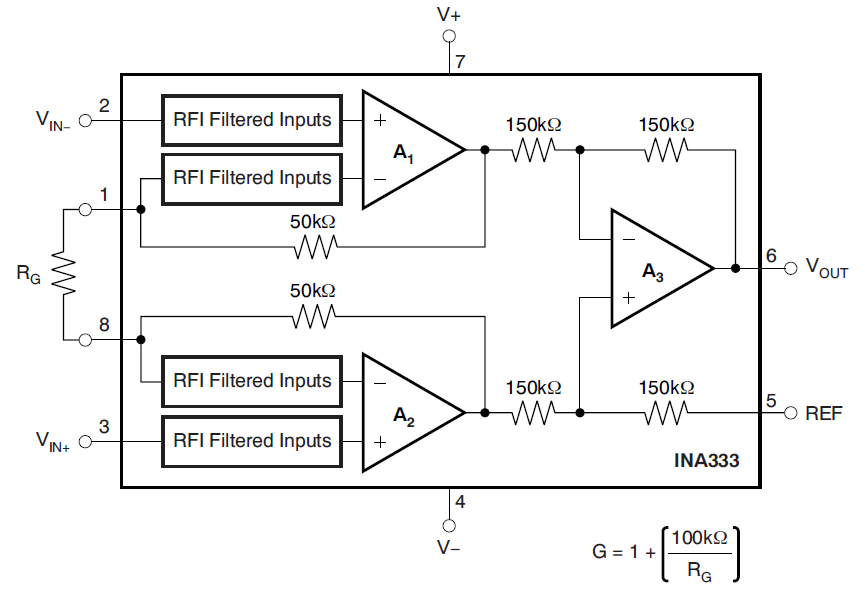
\includegraphics[width=0.8\textwidth]{INA333.png}
\caption{INA333}
\end{figure}
INA333是一款可以使用单电源供电的仪表放大器,相比较INA128使用双电源供电的设计更加科学。在本设计中用于压力传感器桥路放大和人体电阻测量中的微电流放大。

\subsubsection{TS5A3359}
\begin{figure}[H]
\centering
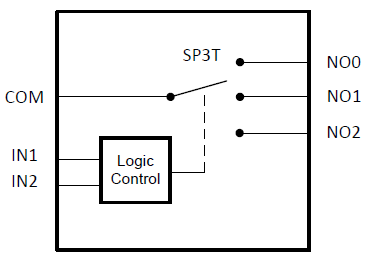
\includegraphics[width=0.4\textwidth]{TS5A3359.png}
\caption{TS5A3359}
\end{figure}
TS5A3359是一款单刀三掷的模拟开关,用于对三路模拟输入进行多路复用。

\subsubsection{TLC0820}
TLC0820是一款并行输出的ADC,片上跟踪保持,使用简便,并行输出可以简化FPGA接口的设计。芯片由实验室提供,用于本设计非常合适。

\subsection{设计细节}
TLC0820的输出电平为5V,与FPGA相连需要注意一些事项。\\

查阅Altera Application Note C51011 (Using Cyclone Devices in Multiple-Voltage Systems),可以得到相关信息。
\begin{figure}[H]
\centering
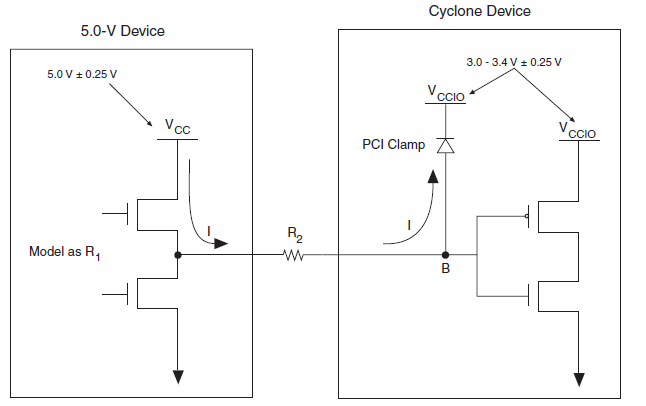
\includegraphics[width=0.6\textwidth]{5V.png}
\caption{Cyclone 5V 电平连接}
\end{figure}
在Cyclone 器件中开启 PCI Clamp,并配合外接电阻$R_2$,使得Cyclone 器件可以兼容5V电平输入。

\section{接口电路设计}
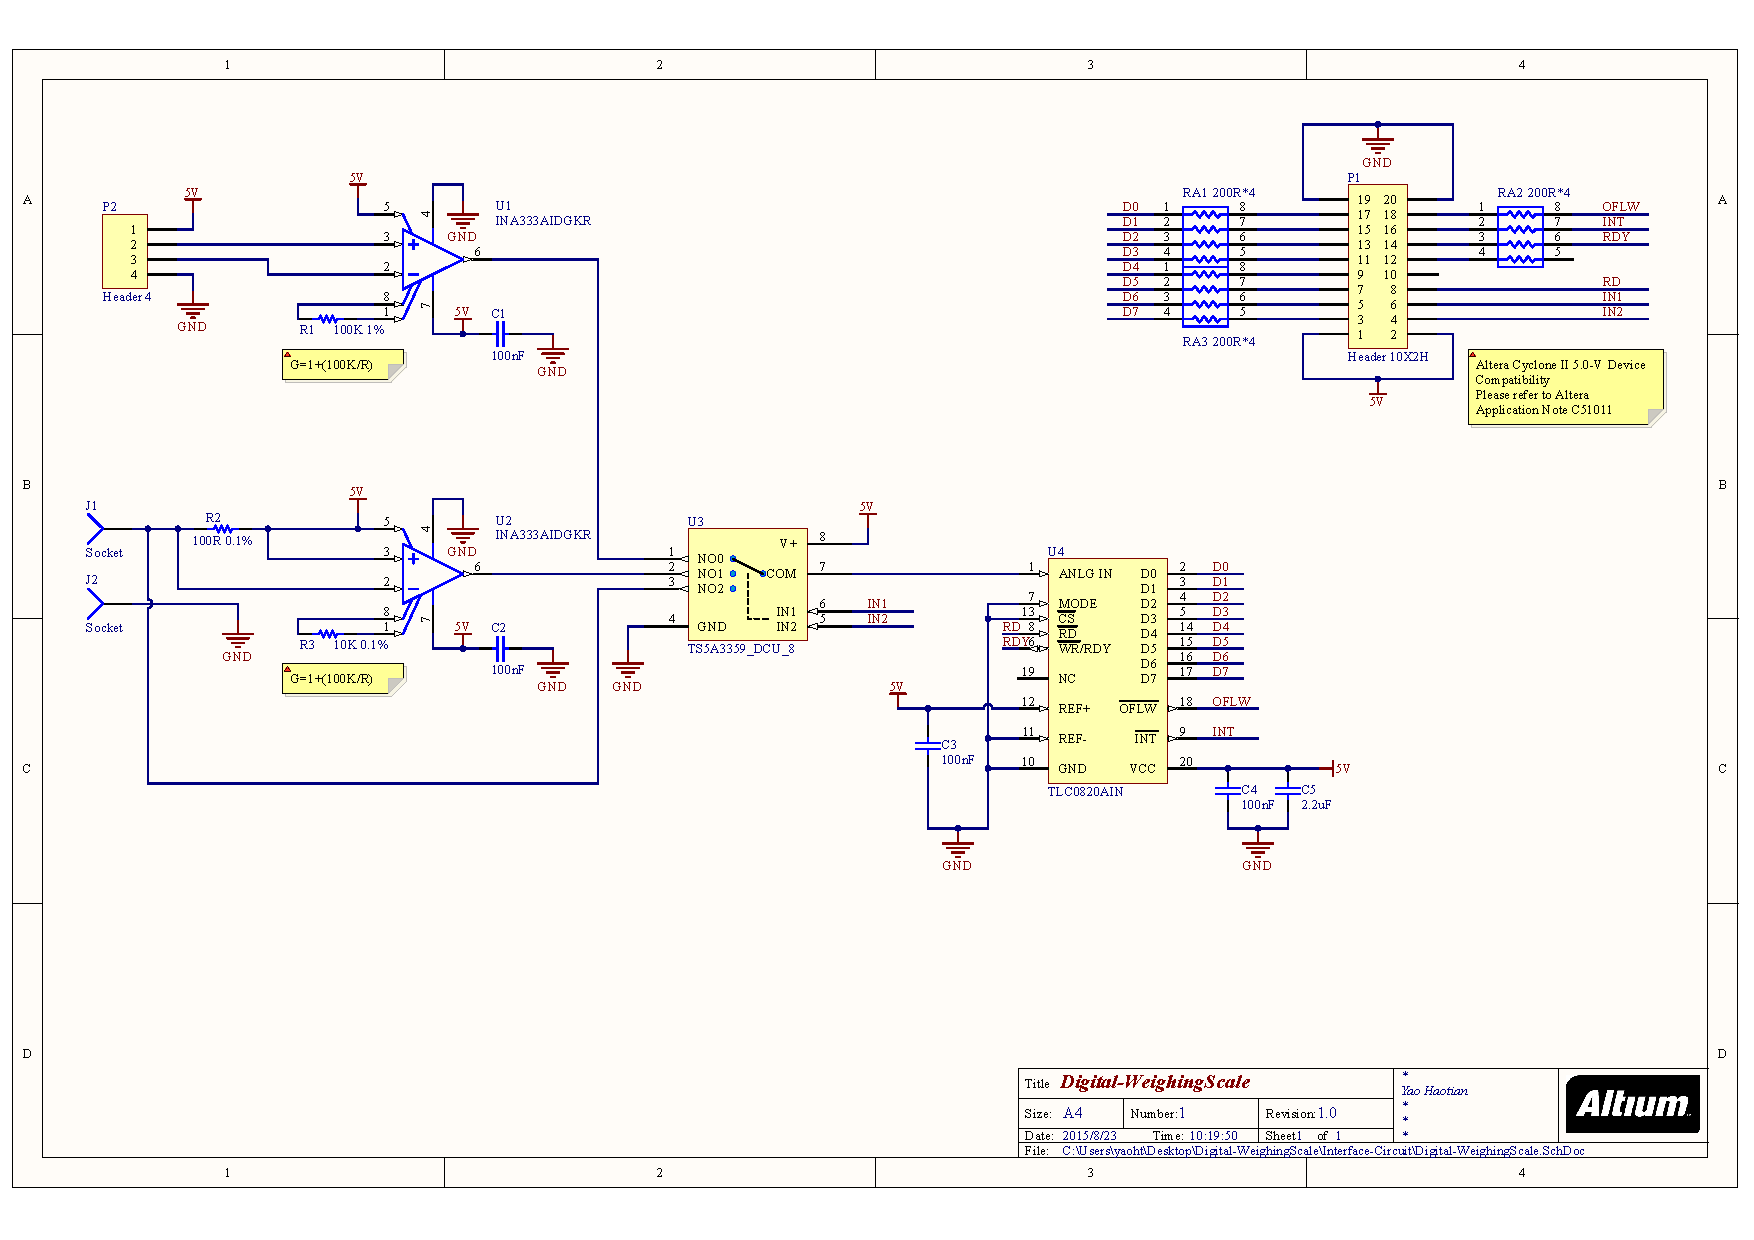
\includepdf[landscape=true]{sch.pdf}
\end{document}
